\chapter{Planificación}

\section{Metodología utilizada}

Incluso desde el inicio de la asignatura Desarrollo Basado en Agentes, el profesor de dicha asignatura D. Luis Castillo Vidal nos exigió el uso de metodologías ágiles para el desarrollo de cada una de las prácticas, que se desarrollaban por grupos generalmente.\\

Para controlar todo el progreso de cada uno de los miembros, el profesor nos facilitó ciertas hojas de cálculo, una para cada grupo, donde cada grupo se encargaría de definir los siguientes elementos:

\begin{itemize}
	\item Cada una de las tareas que se van a llevar a cabo a lo largo de la práctica actual.
	\item Estimación de cuántas horas cada alumno se compromete a dedicar en la práctica actual.
	\item Estimación de cuántas horas cada tarea (o historia) puede ocupar. Es necesario que la suma de esta estimación coincida con la suma de la estimación de horas de cada alumno del grupo.
	\item Registrar las horas dedicadas a cada historia por parte de cada alumno.
	\item Definir, para cada práctica, un miembro del grupo que ejercerá como líder. Es quien debería de mantener las comunicaciones con el profesor.
\end{itemize}

De igual forma, para este proyecto se ha seguido una estrategia similar, que podría definir informalmente como \textit{pseudo-SCRUM}. En los primeros días de definición del proyecto, una vez estaban las bases consensuadas con mi tutor D. Luis Castillo Vidal, también hicimos una sesión de inicio de la metodología, en la que esencialmente llevamos a cabo algunas de las tareas mencionadas anteriormente.\\

Más concretamente, definimos la fecha de comienzo y fin del proyecto, y también definimos una serie de \textit{sprints}, con una cantidad fija de días cada uno tras los cuales organizaríamos una sesión de control para evaluar cómo iba avanzando el proyecto. Además, se consensuaron todas las historias a realizar durante todo el proyecto y se hizo la estimación general en horas.

\section{Temporización}

Antes de comentar en profundidad la temporización, es destacable comentar que inicialmente se realizó una fase de análisis en febrero, por la cual se estipuló dar comienzo al proyecto el día 3 de marzo del presente año y marcarlo como finalizado el día 15 de julio también del presente año, dividido en siete \textit{sprints} de 21 días cada uno a excepción del último. Debido a ciertos problemas, nos vimos obligados a posponer este proyecto y a realizar una nueva fase de replanificación en junio.\\

Durante la fase de análisis del proyecto, se llegó a un consenso con el tutor de establecer como fecha de comienzo el día 7 de junio de 2021 y fecha de finalización del mismo el 14 de septiembre del mismo año. Esta vez, se estipularon diez \textit{sprints} de diez días cada uno.\\

El proyecto se temporizó en 100 unidades de tiempo a completar, donde cada unidad de tiempo equivaldría entre tres y cuatro horas de trabajo real del alumno.\\

También se reestructuraron, en consenso con el tutor, las historias que previamente habíamos considerado para el proyecto en febrero para así ajustar de nuevo el tiempo que teníamos disponible y también teniendo en cuenta el trabajo previo que realicé anteriormente.\\

Surgieron así, 13 tareas o historias que deberían ser completadas a lo largo del periodo planificado anteriormente. En la tabla \ref{tab:historias}, se muestra un resumen de cada historia junto con el tiempo consensuado con el tutor.\\

En dicha tabla no obstante, aparecen 14 historias, y si además sumamos el tiempo estimado para cada una de estas historias, obtendríamos que el total de unidades de tiempo planificadas es de 112 en lugar de 100. Esto se debe a que en febrero, en la fase inicial de análisis, a pesar de que no se pudo seguir adelante con el proyecto, yo como estudiante llevé a cabo algunas tareas de investigación y comprensión que formaban parte de la planificación original, y que no se incluyeron de nuevo en la planificación ya que estaban completadas. Es por eso que se incluyeron de manera adicional indicando el número de horas que ya se había trabajado en el proyecto.

% Please add the following required packages to your document preamble:
% \usepackage{graphicx}
\begin{table}[]
\centering
\resizebox{\textwidth}{!}{%
\begin{tabular}{|l|l|c|}
\hline
\textbf{Historia}                                                                          & \textbf{Descripción}                                                                                                                                                                                                                                                                                                                                                                                                                                & \textbf{Tiempo Estimado} \\ \hline
Completar ciclo de simulador                                                               & \begin{tabular}[c]{@{}l@{}}Leer, interpretar y ejecutar archivos de registro completos. \\ Desde que se analiza cada línea del archivo, \\ hasta que se hace la comunicación con el agente de \\ Telegram.\end{tabular}                                                                                                                                                                                                                             & 7                        \\ \hline
Simular varios receptores                                                                  & \begin{tabular}[c]{@{}l@{}}Probar la recepción de mensajes de Telegram a \\ diferentes usuarios\end{tabular}                                                                                                                                                                                                                                                                                                                                        & 5                        \\ \hline
Procesar entradas de chat \#1                                                              & Identificación de cada usuario usando su cardID                                                                                                                                                                                                                                                                                                                                                                                                     & 5                        \\ \hline
Procesar entradas de chat \#2                                                              & \begin{tabular}[c]{@{}l@{}}Definir opciones de suscripción para notificaciones,\\ siendo capaz de definir:\\ - Recibir o no notificaciones\\ - Si se reciben notificaciones: recibir todas las \\ notificaciones, recibir solo las notificaciones\\ imprescindibles (mensajes de error)\\  o recibir notificaciones de tipo ACL\end{tabular}                                                                                                        & 12                       \\ \hline
Ofrecer progresos individuales                                                             & \begin{tabular}[c]{@{}l@{}}Perfil de progreso individual (o de grupo para aquellas \\ prácticas que sean en grupos)\end{tabular}                                                                                                                                                                                                                                                                                                                    & 7                        \\ \hline
Ofrecer progreso por problema                                                              & Perfil de progreso por un problema concreto                                                                                                                                                                                                                                                                                                                                                                                                         & 5                        \\ \hline
Ofrecer progreso por práctica                                                              & Perfil de progreso por una práctica concreta                                                                                                                                                                                                                                                                                                                                                                                                        & 7                        \\ \hline
Retroalimentaciones simples                                                                & - Fecha de entrega de una práctica concreta                                                                                                                                                                                                                                                                                                                                                                                                         & 6                        \\ \hline
\begin{tabular}[c]{@{}l@{}}Desplegar el sistema a un \\ entorno de producción\end{tabular} & \begin{tabular}[c]{@{}l@{}}Gestionar información en tiempo real, con conexión \\ directa a la base de datos y con agentes reales.\\ Verificar todas las historias previas.\end{tabular}                                                                                                                                                                                                                                                             & 15                       \\ \hline
Procesar entradas de chat \#3                                                              & \begin{tabular}[c]{@{}l@{}}Comprobar el estado de los agentes. Informar\\  al profesor a través de Telegram si uno de los \\ agentes no se encuentra disponible.\end{tabular}                                                                                                                                                                                                                                                                       & 5                        \\ \hline
Documentación                                                                              & Elaboración de la memoria                                                                                                                                                                                                                                                                                                                                                                                                                           & 16                       \\ \hline
Presentación                                                                               & Elaboración de la presentación para la defensa del proyecto                                                                                                                                                                                                                                                                                                                                                                                         & 10                       \\ \hline
Trabajo previo (desde febrero)                                                             & \begin{tabular}[c]{@{}l@{}}En resumen:\\ - Lectura de manuales de JADE\\ - Análisis y comprensión de proyectos relacionados con \\ \textit{behaviours} para entender mejor su funcionamiento\\ - Análisis y comprensión de la arquitectura LARVA\\ - Estudio de agentes y componentes concretos: ConfigFile, \\ Logger, ACLMessageQueue, ACLMSplitQueue,\\  Jerarquía de agentes...\\ - Estudio de la API de Telegram\end{tabular} & 12                       \\ \hline
\end{tabular}%
}
\caption{Backlog de historias estimadas para el proyecto. Cada unidad de tiempo corresponde a 3-4 horas de trabajo real del alumno.}
\label{tab:historias}
\end{table}

\section{Seguimiento del desarrollo}

El seguimiento de cada uno de los \textit{sprints} y de cada una de las tareas se realizó mediante una hoja de cálculo alojada en Google Drive, la cual fue puesta a punto y configurada por el tutor de este proyecto, adaptándola a las necesidades concretas del mismo.\\

La finalidad de esta hoja de cálculo es controlar el número de horas que se dedican a cada una de las historias, en cada uno de los diez \textit{sprints} que se estipularon. De esta forma y gracias a las configuraciones realizadas por el tutor, es posible ver de una forma muy visual el progreso tanto del proyecto a nivel general como del \textit{sprint} que se desee, como se muestra en la figura \ref{img:sprint3}.\\

\begin{figure}[h]
\centering
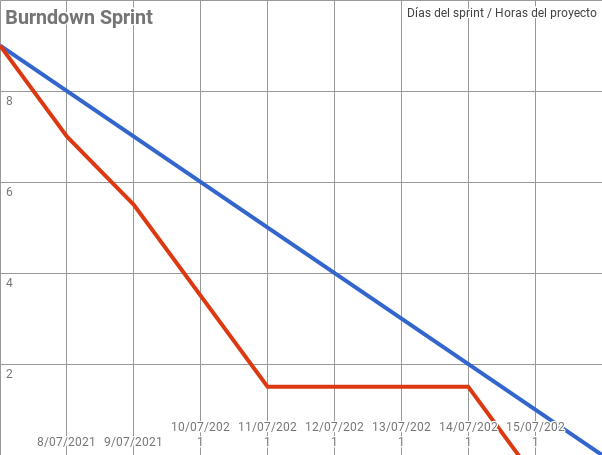
\includegraphics[width=0.9\textwidth]{logos/sprint4.png}\\[1.4cm]
\caption{Progreso del \textit{sprint} número 3. La línea azul representa el progreso ideal, mientras que la línea roja es el progreso real del estudiante durante ese \textit{sprint}.}
\label{img:sprint3}
\end{figure}

Como estudiante, me gustaría destacar que este procedimiento para llevar la cuenta de todas las horas dedicadas al proyecto resulta muy eficiente, ya que constantemente se obtiene retroalimentación real de cuánto va avanzando el proyecto, tanto a nivel general como a nivel concreto de historias.

\section{Diagrama de Gantt}

A continuación, en la figura \ref{img:gantt}, se presenta un diagrama de Gantt en el que se puede apreciar el trabajo realizado durante cada sprint en las distintas tareas previamente mencionadas.

\begin{figure}[h]
\centering
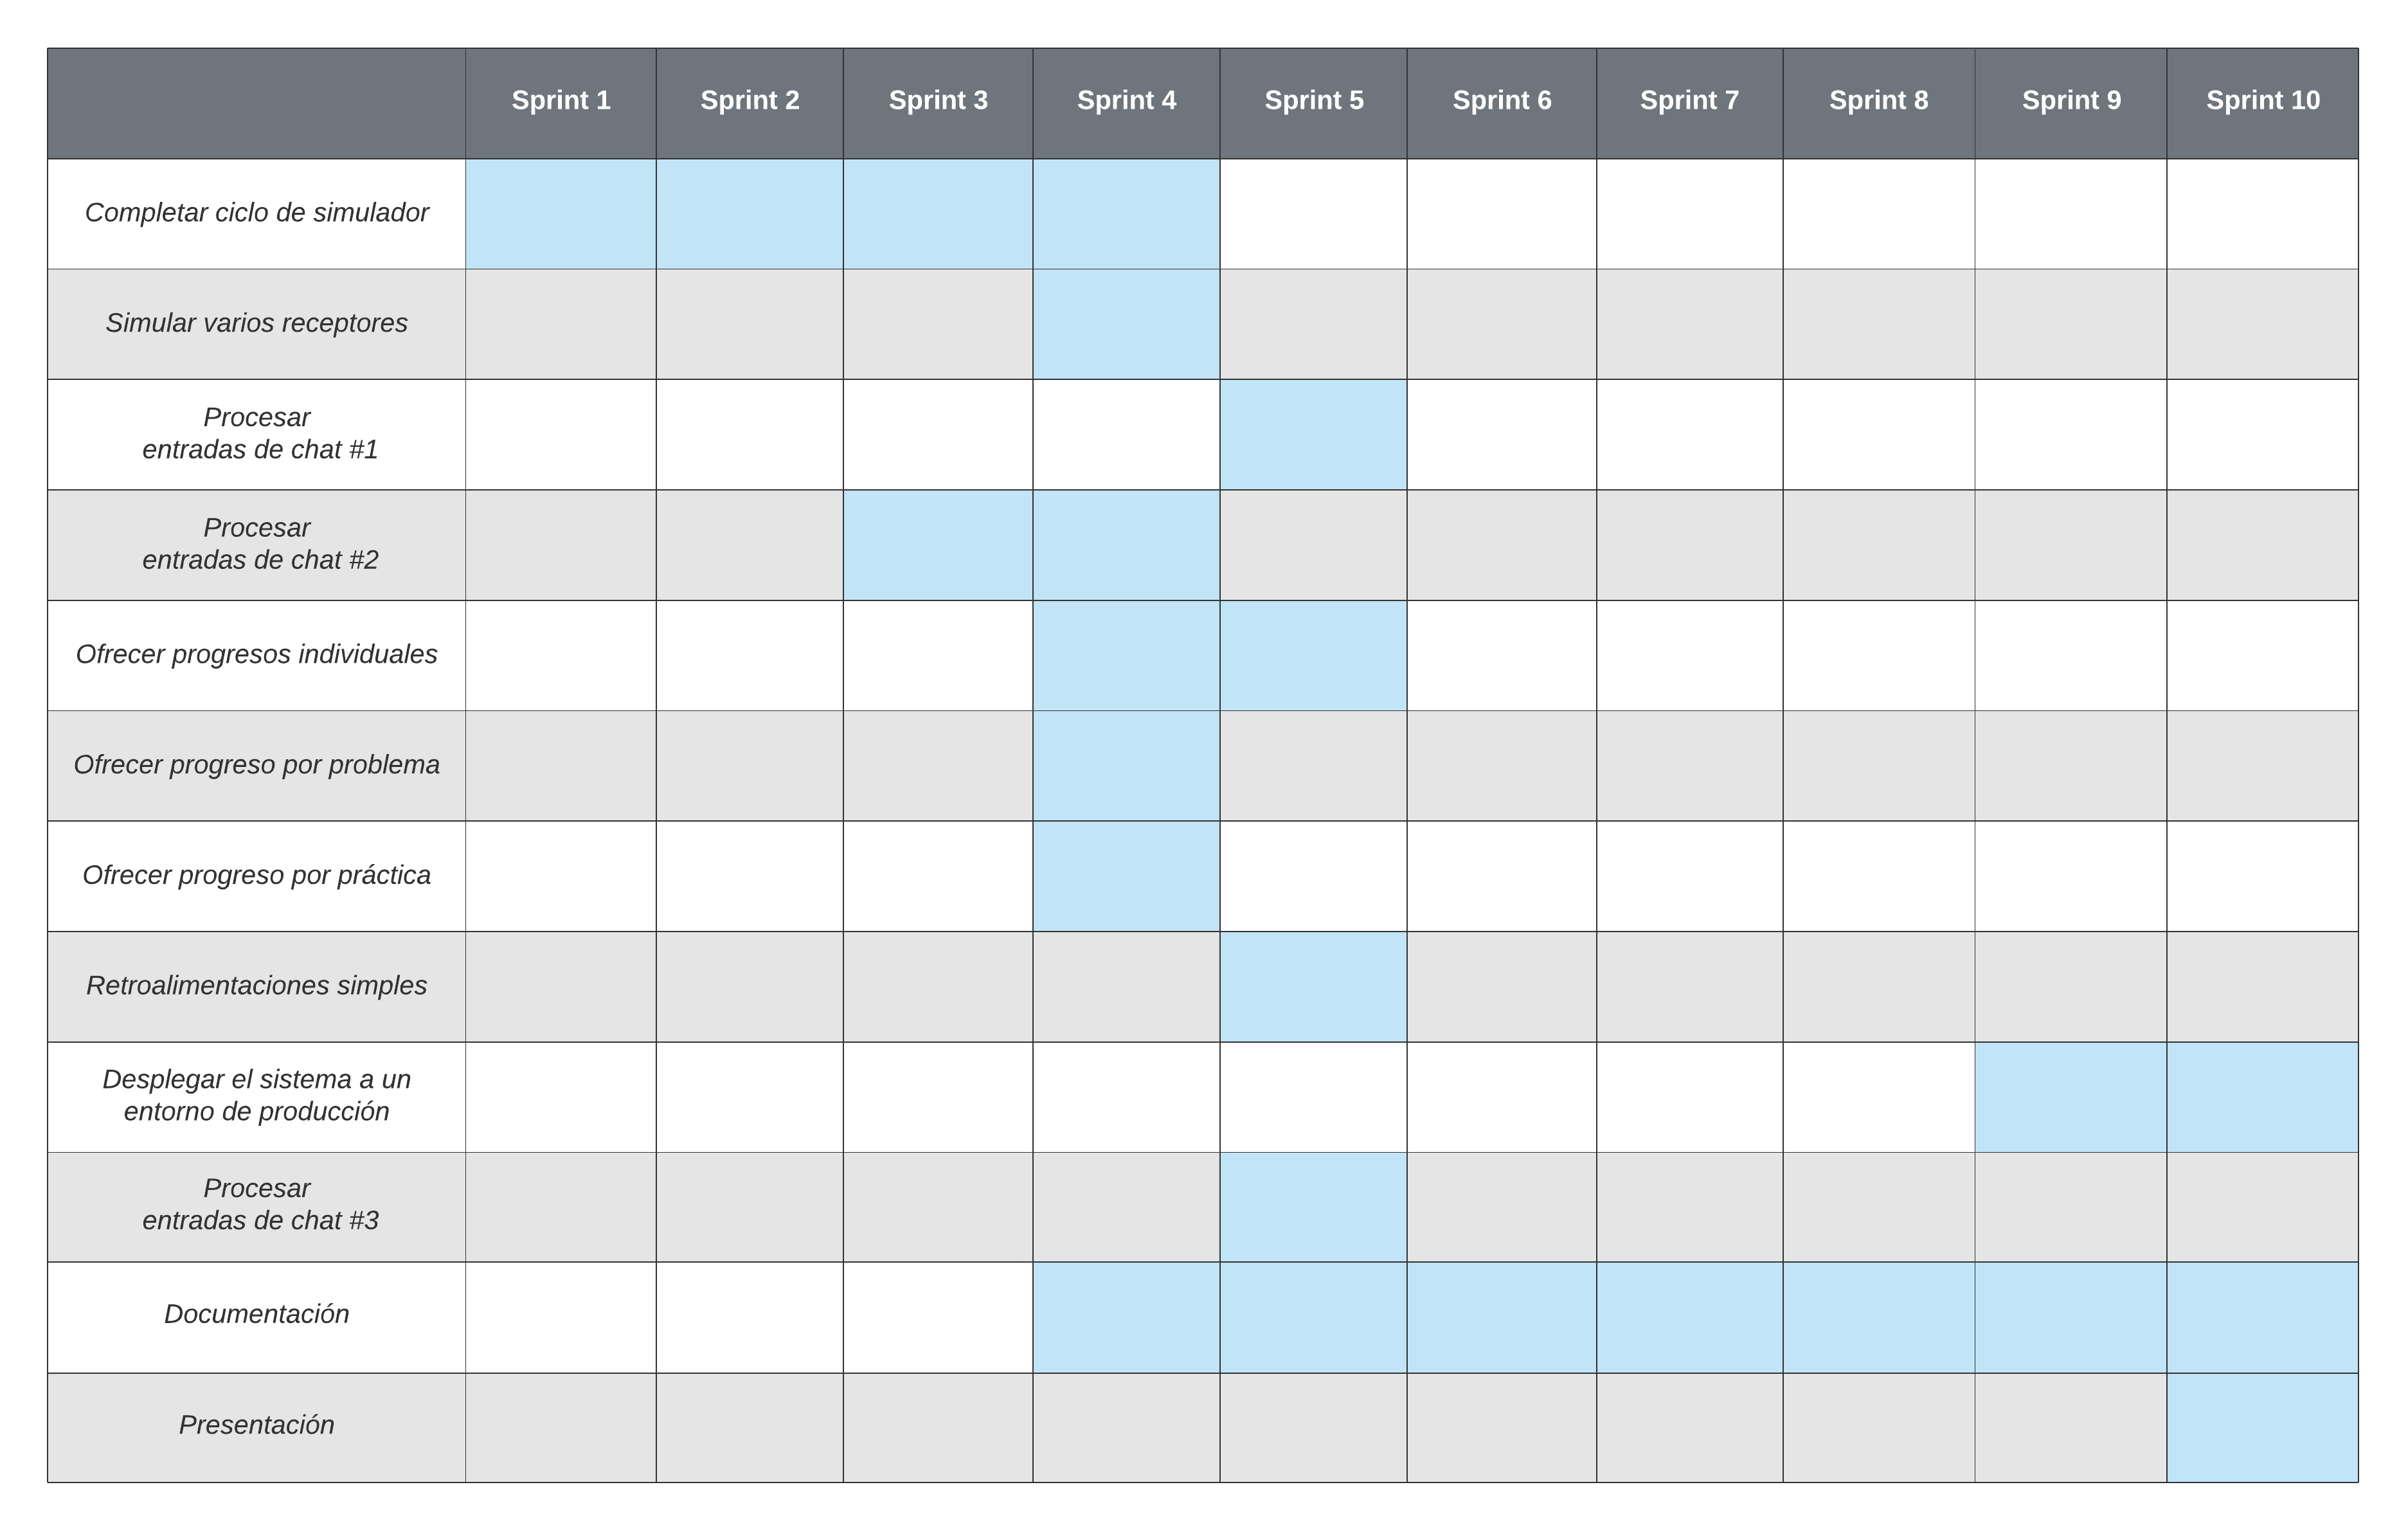
\includegraphics[width=1.1\textwidth]{logos/gantt.png}\\[1.4cm]
\caption{Diagrama de Gantt de la planificación}
\label{img:gantt}
\end{figure}

\section{Recursos}

\subsection{Recursos Humanos}

Los recursos humanos que han intervenido en la realización de este proyecto han sido, como autor del mismo, Francisco Domínguez Lorente y como tutor y supervisor del proyecto, D. Luis Castillo Vidal.

\subsection{Recursos Hardware}

Se han utilizado principalmente dos equipos durante el desarrollo del proyecto, ambos propiedad del autor del mismo, en este caso Francisco Domínguez Lorente:\\

\begin{itemize}
	\item Ordenador personal de sobremesa con procesador AMD Ryzen 5 3600 BOX, tarjeta gráfica Sapphire Radeon RX580 Nitro+, 16GB de memoria RAM y sistema operativo Ubuntu 20.04
	\item Dispositivo móvil Xiaomi Mi 9T Pro con la aplicación Telegram instalada
\end{itemize}

\subsection{Recursos Software}

Con respecto a los recursos a nivel de software que han sido usados en el proyecto, algunos ya han sido mencionados y otros se comentarán con más detalle en el siguiente capítulo. A saber, son:\\

\begin{itemize}
	\item Entorno de desarrollo NetBeans 12. Licencia libre.
	\item Librerías proporcionadas por el tutor del proyecto: LARVA, JADE, JDK
	\item Git y GitHub para el control de versiones
	\item Ubuntu 20.04 y Android 11 como sistemas operativos
	\item Telegram, en sus versiones para móvil y para ordenador
\end{itemize}

\subsection{Estimación de costos}

Con respecto a los recursos humanos, dentro del plan de estudios de la titulación, este propyecto tiene una carga lectiva de 12 créditos ECTS. Lo cual, sabiendo que cada crédito ECTS equivale a 25 horas, se puede traducir en aproximadamente 300 horas de trabajo.\\

Según la Universidad Europea \cite{universidad-europea-2021}, el salario de un ingeniero informático puede oscilar entre los 1.000 y 1.200 euros netos mensuales, por lo cual tomaré de referencia una cuantía de 8 euros netos por hora. Al haber sido estimado este proyecto 300 horas, el coste total de los recursos humanos será de 2.400 euros netos.\\

A continuación, con respecto a los recursos hardware, es necesario realizar ciertas estimaciones sobre la amortización de los dispositivos para saber cuánto coste han supuesto los mismos durante toda la duración del proyecto. Usaremos como referencia la tabla de coeficientes de amortización lineal proporcionada por la Agencia Tributaria \cite{amortizacion-agencia-tributaria}.\\

El primer dispositivo hardware, el ordenador personal, tuvo un coste final de 1000 euros. El periodo de amortización para sistemas informáticos es de 6 años, lo cual quiere decir que cada año se estima un coste de 166,67 euros del dispositivo. Al haberse desarrollado este proyecto durante los meses de febrero y septiembre \textit{(aproximadamente 7 meses)}, el coste estimado del dispositivo para el proyecto será de 97,25 euros.\\

De igual forma, el dispositivo móvil tuvo un coste final de 330 euros. Siguiendo las mismas indicaciones que en el párrafo anterior, el coste estimado del dispositivo para este proyecto habrá sido de 32 euros.\\

Los recursos software no han implicado costes adicionales, ya que todos ellos han sido obtenidos de manera gratuita siguiendo las indicaciones de las licencias de los mismos.\\

Así pues, se estima que el coste total del proyecto será de 2.529,25 euros sin tener en cuenta gastos adicionales como pueden ser la conexión a internet o el consumo de electricidad de los dispositivos, que pueden ser más complicados de calcular y de estimar.